\chapter{Resultados e Discussão}
\label{ch:resultados_discussao}

\textit{\textcolor{red}{Fazer um parágrafo introdutório sobre o capítulo.}}

\section{Tópico 1}
\label{sec:topico_1}

\textit{\textcolor{red}{Neste item o aluno deve apresentar os resultados obtidos no estudo. Lembre-se que deve responder os objetivos do estudo. Além de apresentar os resultados, o aluno deve discuti-los e comparar com os resultados obtidos por outros autores. A discussão deve ser fundamentada cientificamente e tecnicamente. Use Figuras e Tabelas para a apresentação e discussão dos resultados. Siga os modelos de discussão de artigos.}}

De acordo com a Tabela \ref{tab:exemplo_tabela} ...

\begin{table}[!ht]
	\caption{Exemplo de tabela}
	\centering
	\begin{tabular}{l|c}
		\hline
        \textbf{Métrica} & \textbf{Valor} \\ \hline 
        \textbf{MSE} & 10188,0654 \\ \hline 
        \textbf{MAE} & 65,5954 \\ \hline 
        \textbf{R$^2$} & 0,9682 \\ \hline 
        \textbf{r} & 0,9840 \\ \hline
        \textbf{Fator de 2} & 1,0000 \\ \hline
	\end{tabular}
	\fdp
	\label{tab:exemplo_tabela}
\end{table}

\section{Tópico 2}
\label{sec:topico_2}

\textit{\textcolor{red}{Os resultados e discussão podem ser subdivididos em tópicos ou ser apresentado de forma conjunta.}}

De acordo com Figura \ref{fig:fig_exemplo_imagem3} ...

\begin{figure}[!h]
    \caption{Exemplo de imagem.}
    \centering
    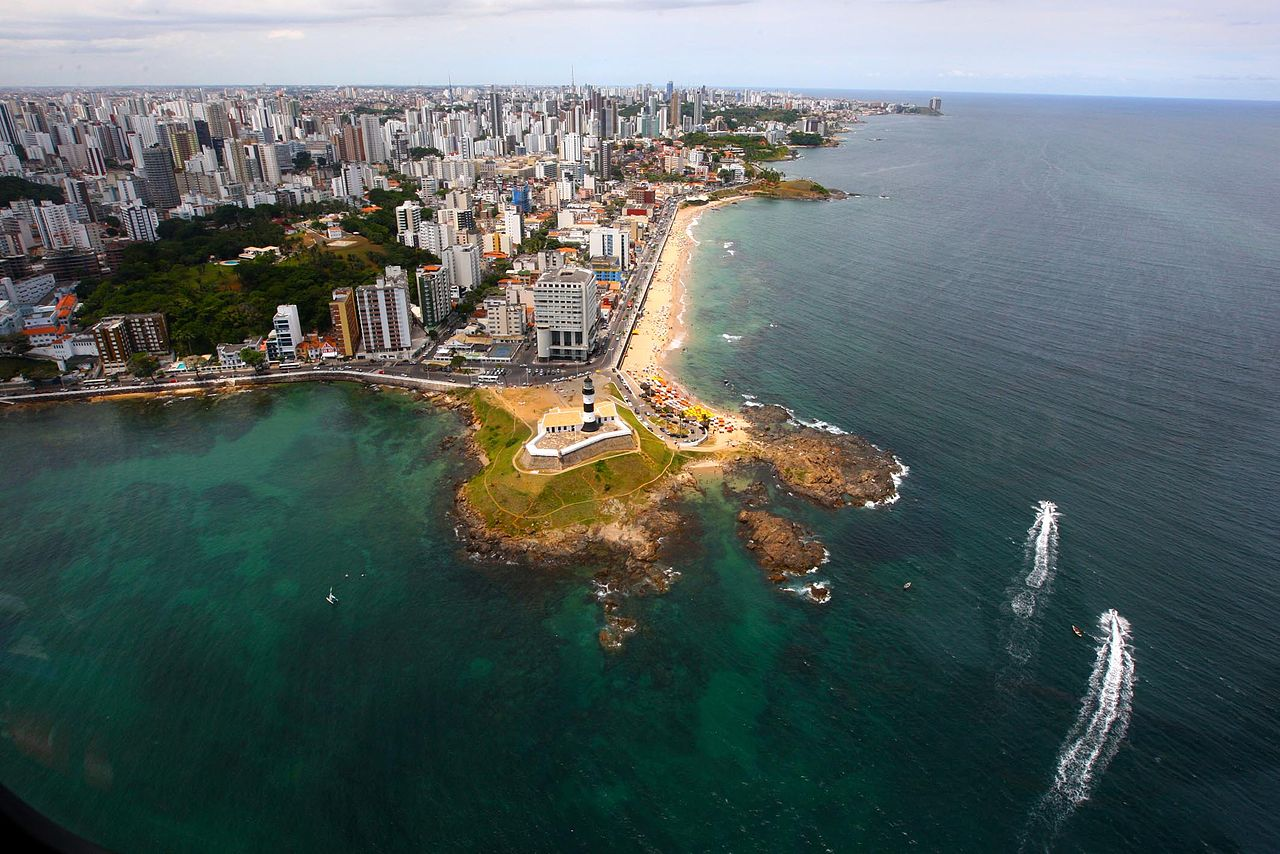
\includegraphics[width=0.45\textwidth]{images/farol_da_barra.jpg}
    \fol{hunter2007matplotlib}
    \label{fig:fig_exemplo_imagem3}
\end{figure}